\section{Building NWAs from other NWAs (namespace \texttt{wali::nwa::construct})}
\label{Se:Building NWAs}

The library provides functions for performing automata-theoretic operations upon
NWAs. The supported operations are union, intersection, concatenation,
reversal, Kleene star, complement, and determinization.

The library supports two interfaces to each of these operations. In one, the
operation allocates an NWA with \texttt{new}, performs the construction, and
returns a \texttt{NWARefPtr} to the result.  In the other, the operation takes
a reference to an NWA, clears it, and constructs the result in-place. The
first form is usually more convenient to use, and creates a mini language for
set expressions; the second form makes it possible to store the result of an
operation in a subclass of \texttt{NWA}.

Each of these functions is in the namespace \texttt{wali::nwa::construct}:

\begin{functionlist}

  \functionitem[\texttt{NWARefPtr unionNWA( NWA const \& a, NWA const \& b )}]
  \functionitem[\texttt{void unionNWA( NWA \& out, NWA const \& a, NWA const \& b )}]
    Computes the union of the NWAs \texttt{a} and \texttt{b},
    either returning the result or storing it in \texttt{out}.
    See Section
    \ref{Se:Union}. (This function is called \texttt{unionNWA} instead of
    \texttt{union} because the latter is a keyword.) The two NWAs must not
    have any states in common, and the output will be nondeterministic even
    if both input NWAs are deterministic. The running time is
    $O(|Q^a|+|Q^b|+|\delta^a|+|\delta^b|)$.

  \functionitem[\texttt{NWARefPtr intersect( NWA const \& a, NWA const \& b )}]
  \functionitem[\texttt{void intersect( NWA \& out, NWA const \& a, NWA const \& b )}]
    Computes the intersection of the NWAs \texttt{a} and \texttt{b},
    either returning the result or storing it in \texttt{out}.
    See Section \ref{Se:Intersection}. If both input NWAs are deterministic,
    the output will be deterministic. The worst-case running time is
    $O(|Q^a||Q^b|d_ad_b)$, where $d_a$ is the maximum out-degree
    of a state in \texttt{a} and $d_b$ is the maximum out-degree of a state
    in \texttt{b}.

  \functionitem[\texttt{NWARefPtr concat( NWA const \& left, NWA const \& right )}]
  \functionitem[\texttt{void concat( NWA \& out, NWA const \& left, NWA const \& right )}]
    Computes the concatenation of the NWAs \texttt{left} and
    \texttt{right}, either returning the result or storing it in
    \texttt{out}.
    See Section \ref{Se:Concatenation}. The output automaton will be
    nondeterministic. The running time is
    $O(|Q^a|+|Q^b|+|\delta^a|+|\delta^b|+|Q^a||\delta_r^b|)$.
    (The $\delta_r^b$ term can be refined even further to be the number of
    return transitions with a state from $Q_0^b$ in the call predecessor
    position.)

  \functionitem[\texttt{NWARefPtr star( NWA const \& orig )}]
  \functionitem[\texttt{void star( NWA \& out, NWA const \& orig )}]
    Computes the Kleene-Star of the NWA \texttt{orig}, either
    returning the result or storing it in \texttt{out}. See Section
    \ref{Se:Star}. The output automaton will be nondeterministic. The
    running time is $O(|Q|+|\delta|+|Q_0||Q_f||\delta_c|)$.

  \functionitem[\texttt{NWARefPtr reverse( NWA const \& orig )}]
  \functionitem[\texttt{void reverse( NWA \& out, NWA const \& orig )}]
    Computes the NWA that accepts the reverse of each nested word
    accepted by the NWA \texttt{orig}, either returning the result or
    storing it in \texttt{out}. See Section \ref{Se:Reverse}. The running
    time is $O(|Q|+|\delta|)$.

  \functionitem[\texttt{NWARefPtr determinize( NWA const \& orig )}]
  \functionitem[\texttt{NWARefPtr determinize( NWA \& out, NWA const \& orig )}]
    Computes a determinization of \texttt{orig}, either returning the
    result or storing it in \texttt{out}.
    See Section \ref{Se:Determinize}. The worst-case running time for this
    algorithm is at least $O({|Q|^3} \cdot2^{|Q|^2})$.

  \functionitem[\texttt{NWARefPtr complement( NWA const \& orig, bool determinize )}]
  \functionitem[\texttt{void complement( NWA \& out, NWA const \& orig, bool determinize )}]
    Computes the complement of the determinization of \texttt{orig},
    either returning the result or storing it in \texttt{out}.
    See Section
    \ref{Se:Complement}. For complementing the set of final states to work
    correctly, two things must hold: \texttt{orig} must be deterministic and
    the transition functions must be total. (That is, for a given state $q$
    and symbol $\sigma$, there must be exactly one internal transition $(q,
    \sigma, q') \in\delta_i$, exactly one call transition $(q, \sigma,
    q')\in\delta_c$, and exactly one return transition $(q, p, \sigma,
    q')\in\delta_r$ for each state $p$.)

    \vspace{0.5\baselineskip}
    If \texttt{determinize} is \texttt{true}, it will
    automatically determinize the input NWA before complementation, which
    also guarantees the input machine will be total. If you
    know that \texttt{orig} is already deterministic and total, you can set
    \texttt{determinize} to
    \texttt{false} to avoid this step. (Complementing a nondeterministic or
    non-total NWA can easily lead to an incorrect result.) If
    \texttt{determinize} is \texttt{true}, the worst-case running time is the
    same as for the \texttt{determinize} function (roughly
    $O(2^{|Q|^2})$). If \texttt{determinize} is \texttt{false}, the running
    time is $O(|Q|+|\delta|)$.

\end{functionlist}

As mentioned above, these functions create a small language of set
expressions. For instance, to compute an automaton \texttt{M} whose language
is $\texttt{A} \cup (\texttt{B} \cap \texttt{C})*$ (where \texttt{A},
\texttt{B}, and \texttt{C} are \texttt{NWARefPtr}s), one can write
\begin{center}
  \texttt{NWARefPtr M = unionNWA(*A, *star(*intersect(*B, *C)))}
\end{center}


\begin{figure}[tb]
  \centering
  \begin{minipage}{0.49\textwidth}
    \centering
    \nwaimage[.49]{Figures/figure-1}
    \caption{An example NWA.}
    \label{Fi:Example1}
  \end{minipage}
  \begin{minipage}{0.49\textwidth}
    \centering
    \nwaimage[0.49]{Figures/union-other}
    \caption{A second example NWA.}
    \label{Fi:Union1}
  \end{minipage}
\end{figure}

\begin{figure}[tbp]
  \centering
    \nwaimage[.55]{Figures/union-result}
  \caption{The NWA resulting from the union of the NWA in Figure
    \ref{Fi:Example1} and the NWA in Figure \ref{Fi:Union1}. Note that there
    are two initial states.}
  \label{Fi:Union2}
\end{figure}



\subsection{Union}
\label{Se:Union}
The union of two NWAs is constructed by taking the union of each of the
components of the NWAs. (In
particular, it does \textsl{not} do a cross-product construction, and will
\textsl{always} produce a nondeterministic automaton as a result as long as
both machines have at least one initial state.)

Formally, given $N$ and $M$ such that
\begin{itemize}
 \item $N = (Q_N, \Sigma_N, Q_{0,N}, \delta_N, F_N)$
 \item $M = (Q_M, \Sigma_M, Q_{0,M}, \delta_M, F_M)$
\end{itemize}
then the union is computed as follows:
\begin{itemize}
 \item $N \cup M = (Q_N \cup Q_M, \Sigma_N \cup \Sigma_M, Q_{0,N} \cup
   Q_{0,M}, \delta_N \cup \delta_M, F_N \cup F_M)$
\end{itemize}

As an example, \figref{Union2} illustrates the union of \figref{Example1} and
\figref{Union1}.


The state sets of the NWAs must not overlap,
i.e., $Q_1 \cap Q_2 = \emptyset$. \textsl{Client code should not rely on
  this condition being checked} or any particular behavior occurring if it
does not hold.

Client information is copied directly from the original NWAs using
\texttt{ClientInfo::clone()}.


\subsection{Intersection}
\label{Se:Intersection}

The intersection of two NWAs is computed in the standard cross-product
fashion, using a worklist algorithm to only compute those states that
are reachable.

The algorithm traverses the original NWAs starting at
the initial states and incrementally adds transitions for each pair of
``intersectable'' transitions that are encountered. By default, transitions
are intersectable when the transitions are the same kind (internal, call,
or return) and the symbols on the edge are identical or one is wild.

For example, \figref{Intersect1} shows the intersection of \figref{Example1} and
\figref{Intersect1}, and \figref{Intersect4} shows the intersection of the
two NWAs in \figref{Intersect3}.

 
\begin{figure}[tp]
  \centering
  \begin{minipage}{0.49\textwidth}
    \centering
    \nwaimage[0.45]{Figures/intersection-simple-other}
    \caption{Simple NWA to intersect with the NWA in Figure \ref{Fi:Example1}.}
    \label{Fi:Intersect1}
  \end{minipage}
  \begin{minipage}{0.49\textwidth}
    \centering
    \nwaimage{Figures/intersection-simple-result}
    \caption{The NWA resulting from the intersection of the NWA in Figure
      \ref{Fi:Example1} and the NWA in Figure \ref{Fi:Intersect1}.}
    \label{Fi:Intersect2}
  \end{minipage}
\end{figure}

\begin{figure}[p]
  \centering
    \adjustbox{width=\textwidth,height=\textheight,keepaspectratio=true}{
    \nwaimage{Figures/intersection-complex-first}
    \nwaimage{Figures/intersection-complex-second}}
  \caption{Two complex NWAs to intersect.}
  \label{Fi:Intersect3}
\end{figure}

\begin{figure}[p]
  \centering
    \nwaimage[.45]{Figures/intersection-complex-result}
  \caption{The NWA resulting from the intersection of the NWAs in Figure \ref{Fi:Intersect3}.}
  \label{Fi:Intersect4}
\end{figure}

\antistupidfloats

It is possible to customize what symbols are considered equivalent, or
otherwise impose constraints on what transitions can be intersected, by
overriding the \texttt{transitionIntersect} function in a subclass of
\texttt{NWA}. In addition, it is possible to impose additional constraints on
what states can be combined by overriding \texttt{stateIntersect}. Both
functions also produce the result of the intersection:
\texttt{transitionIntersect} produces the symbol that will be used on the
resulting edge, and \texttt{stateIntersect} produces the state that will be
used as the target.

The default behavior of
\texttt{transitionIntersect} is that two transitions are intersectable if
neither symbol is epsilon and either the symbols are the same or at least one of
the symbols is a wild. (Epsilon transitions are dealt with in
\texttt{intersect()} itself. If you override \texttt{transitionIntersect}, it
should return \texttt{false} if either input is epsilon.)

The default behavior of \texttt{stateIntersect} is that any two
states can be combined, the resulting state is labeled with a
\texttt{Key} that is uniquely generated from the pair of the \texttt{Keys} of
the two states under consideration, and the client information associated
with the resulting state is \texttt{null}.


Client information is initially generated by the helper method \texttt{stateIntersect},
but can be altered through the use of the helper methods
\texttt{intersectClientInfoInternal}, \texttt{intersectClientInfoCall}, and
\texttt{intersect\-Client\-InfoReturn}, which are invoked by
\texttt{intersect()} as transitions of the three different kinds involving the
associated state are added.  The default behavior of these three functions is
to perform no changes to the \texttt{ClientInfo}.  These methods can be
overridden in subclasses to specify alternative behaviors.

\goodbreak
The following operations are virtual functions in class \texttt{NWA} and are intended
to be overridden to customize behavior:

\begin{functionlist}

  \functionitem[\texttt{bool stateIntersect(
                  \parbox[t]{4in}
                              {NWA const \& first, Key state1,\\ 
                               NWA const \& second, Key state2,\\
                               Key\& resSt, ref\_ptr<ClientInfo>\& resCI)}}]
    Determines whether the given states can be combined and,
    if so, creates the combined state. If the two states are incompatable,
    returns \texttt{false}. If the two states are compatable, it computes the
    key of the combined state (storing it in \texttt{resSt} and the client
    information (storing it in \texttt{resCI}), then returns \texttt{true}.

  \functionitem[\texttt{bool transitionIntersect(
                  \parbox[t]{4in}
                              {NWA const \& first, Key sym1,\\
                               NWA const \& second, Key sym2,\\ 
                               Key\& resSym )}}] \nopagebreak
    Determines whether the given symbols are considered to be equivalent for
    the purposes of intersection. If so, it computes the symbol that should
    be associated with the combined transition (storing it in
    \texttt{resSym}) and returns true. If not, returns false.

  \functionitem[\texttt{void intersectClientInfoInternal(
                  \parbox[t]{4in}
                     {NWA const \& first, Key src1, Key tgt1,\\
                      NWA const \& second, Key src2, Key tgt2,\\
                      Key resSym, Key resSt )}}]
    \nopagebreak
  \functionitem[\texttt{void intersectClientInfoCall(
                  \parbox[t]{4in}
                      {NWA const \& first ,Key call1, Key entry1,\\
                       NWA const \& second, Key call2, Key entry2,\\
                       Key resSym, Key resSt )}}] \nopagebreak
  \functionitem[\texttt{void intersectClientInfoReturn(
                  \parbox[t]{4in}
                      {NWA const \& first, Key exit1, Key call1, Key ret1,\\
                       NWA const \& second, Key exit2, Key call2, Key ret2,\\
                       Key resSym, Key resSt )}}]
    Called after a transition of the corresponding type is added to the
    automaton. It is intended to be used to
    alter the client information associated with \texttt{resSt} given the
    endpoints of the new transition.

\end{functionlist}




\subsection{Concatenation}
\label{Se:Concatenation}

The concatenation of two NWAs is constructed by taking the union of all
states and transitions of the two automata, and adding
internal epsilon transitions from each final state of the first NWA to each
initial state of the second NWA.  In the resulting NWA, the initial states
are the initial states from the first NWA, and the final states are the final
states of the second NWA.

However, the Kleene-star construction is a bit more complicated just this,
because we need to address the issue of an unbalanced-left
word being concatenated with an unbalanced-right word.  (Recall that the
definition of what happens when an NWA reads a pending return is that it is
allowed to take a return transition where the call predecessor is an initial
state of the automaton.) 

To properly deal with the case where the second part is unbalanced
right, the transitions from the second automaton are augmented in the
following manner. When computing the concatenation of \texttt{left} and
\texttt{right}, for each transition $(q, p_0, a, q')
\in\delta_r^{\texttt{right}}$ where $p_0 \in Q_0^\texttt{right}$, and each $q
\in Q^\texttt{left}$, we add $(p, q, a, q')$ to $\delta_r$ of the result.


 % If the original NWAs are $(Q_1, \Sigma_1,
%{Q_0}_1, \delta_1, {Q_f}_1)$ and $(Q_2, \Sigma_2, {Q_0}_2, \delta_2,
%{Q_f}_2)$, then the resulting NWA is $(Q, \Sigma, Q_0, \delta, Q_f)$ where $Q
%= Q_1 \cup Q_2$, $\Sigma = \Sigma_1 \cup \Sigma_2$, $Q_0 = {Q_0}_1$, $\delta
%= \delta_1 \cup \delta_2 \cup \delta_\epsilon$ (where $\delta_\epsilon =
%\{(q,\epsilon,q') | q \in {Q_f}_1, q' \in {Q_0}_2\}$, and $Q_f = {Q_f}_2$ .
%The NWA resulting from the concatenation of the NWA in Figure
%\ref{Fi:Example1} and the NWA shown in Figure \ref{Fi:Concat1} is shown in
%Figure \ref{Fi:Concat2}.

\begin{figure}[p]
  \centering
  \begin{minipage}{0.5\textwidth}
    \begin{minipage}{\textwidth}
      \centering
      \nwaimage[1]{Figures/concat-other}
      \caption{Simple NWA to concatenate onto the NWA in Figure \ref{Fi:Example1}.}
      \label{Fi:Concat1}
    \end{minipage}

    \vspace{2\baselineskip}
    \begin{minipage}{0.8\textwidth}
      \centering
      \nwaimage[0.55]{Figures/reverse-of-figure-1}
      \caption{The NWA resulting from performing reverse on the NWA in Figure \ref{Fi:Example1}.}
      \label{Fi:Reverse1}
    \end{minipage}
  \end{minipage}
  \begin{minipage}{0.49\textwidth}
    \centering
    \nwaimage[0.75]{Figures/concat-result}
    \caption{The NWA resulting from the concatenation of the NWA in Figure
      \ref{Fi:Example1} with the NWA in Figure \ref{Fi:Concat1}.}
    \label{Fi:Concat2}
  \end{minipage}
\end{figure}

\antistupidfloats



The state sets of the NWAs must not overlap,
i.e., $Q_1 \cap Q_2 = \emptyset$. \textsl{Client code should not rely on
  this condition being checked} or any particular behavior occurring if it
does not hold.

Client information is copied directly from the original NWAs using
\texttt{ClientInfo::clone()}.

\figref{Concat2} shows the result of concatenating \figref{Example1} and
\figref{Concat1}.


\subsection{Kleene-Star}
\label{Se:Star}

Like concatenation, Kleene-star is complicated in the case of NWAs because of
the ability to have unbalanced-right words in the automaton's
language. Relative to standard FAs, in the concatenation case we only needed
to add extra transitions; in this case, we must add additional states as well.

When computing $R = A*$ for some
NWA $A$, the resulting NWA has two ``copies'' of $A$. These are denoted by
primed and unprimed version of states from $A$ in the definition below. 

\begin{figure}[p]
  \centering
    \nwaimage[.4]{Figures/star-simple}
  \caption{An NWA on which to perform Kleene-Star.}
  \label{Fi:Star1}
\end{figure}

\begin{figure}[p]
  \centering
    \nwaimage[1.1]{Figures/star-simple-result}
  \caption{The NWA resulting from performing Kleene-Star on the NWA in Figure \ref{Fi:Star1}.}
  \label{Fi:Star2}
\end{figure}
\antistupidfloats


Suppose $R$ is reading a word $w_1w_2\cdots w_n$ where each $w_i \in
L(A)$. $R$ begins in a start state of $A'$. Henceforth it maintains an
invariant: if the next symbol is in a return position, then that symbol is a
\emph{pending} return iff $R$ is in the $A'$ portion (i.e. if the current state is
primed). Internal transitions thus keep $R$ in the same copy of $A$, and call
transitions always take $R$ to the unprimed copy of $A$ (because if it then
reads a return, the return will match that call). Return transitions can
target either copy of $A$: if the call predecessor is unprimed, then the
target will be unprimed; if the call predecessor is primed, then the target
will be primed.

The description above describes $R$'s operation under ``normal''
conditions. If it is about to move to a final state however, it is also allowed to guess that it
should restart after the current character. This guess is correct if is
reading last character in $w_i$
(making the next character first one in $w_{i+1}$). $R$ is allowed to
restart only if it is about to move to a final state, but that final state
can be in either copy of A. If the machine
does restart, it moves to an initial state (which is always primed, in order to
maintain the invariant).

The NWA resulting from performing Kleene-Star on the NWA shown in
\figref{Star1} is shown in \figref{Star2}.

Formally, if the original NWA is $(Q, \Sigma, Q_0, \delta, Q_f)$,
then the result of performing Kleene-Star on that NWA is $(Q', \Sigma,
Q_0', \delta', Q_0')$ where $\delta' =
\{\delta_i',\delta_c',\delta_r'\}$ using the following rules:

\begin{mathpar}
{\inferrule*[left=\textsc{States}]
         {q \in Q}
  { q \in Q' \\ q' \in Q'}
}
\and
{\inferrule*[left=\textsc{Initial and Final States}]
         {q_0 \in Q_0}
  { q_0' \in Q_0' \\ q_0' \in Q_f' }
} \\
\and
{\inferrule*[left=\textsc{Internal}]
             {(q,a,p) \in \delta_i }
  { (q,a,p) \in  \delta_i' \\ (q',a,p') \in \delta_i'}
}
\and
{\inferrule*
  {(q,a,p) \in \delta_i \\ p \in Q_f \\ r' \in  Q_0'}
  {(q,a,r') \in \delta_i'\\ (q',a,r') \in \delta_i' }
}
\and
{\inferrule*[left=\textsc{Call}]
           { (q,a,p) \in \delta_c  }
  { (q,a,p) \in  \delta_c' \\ (q',a,p) \in \delta_c'   }
}
\and
{\inferrule*
    { (q,a,p) \in \delta_c \\ p \in Q_f \\ r' \in Q_0' }
  { (q,a,r') \in \delta_c'\\ (q',a,r') \in \delta_c' }
}
\and
{\inferrule*[left=\textsc{Return}]
              { (q,r,a,p) \in \delta_r }
  {(q,r,a,p) \in  \delta_r' \\ (q,r',a,p') \in \delta_r' }
}
\and
{\inferrule*
  { (q,r,a,p) \in \delta_r \\ p \in Q_f \\  s' \in Q_0'}
  {(q,r,a,s') \in \delta_r' \\ (q,r',a,s') \in \delta_r'  }
}\\
{\inferrule*
  { (q,r,a,p) \in \delta_r \\ r \in Q_0 \\ s \in Q' }
  {(q',s,a,p') \in  \delta_r' }
}
\and
{\inferrule*
  { (q,r,a,p) \in \delta_r \\ r \in Q_0 \\ s \in Q' \\ p \in Q_f \\ t' \in Q_0'}
  {(q',s,a,t') \in \delta_r' }
}
\end{mathpar}


Client information is copied directly from the original NWA (using
\texttt{ClientInfo::clone()}) such that for each $q \in Q$, $q$
and $q'$ have (different copies of) the same client information.

%Consider the slightly more complex example of computing the Kleene-Star of the NWA shown in Figure \ref{Fi:Star3}.  The resulting NWA is shown in Figure \ref{Fi:Star4}.

%\begin{figure}[htbp]
%  \centering
%    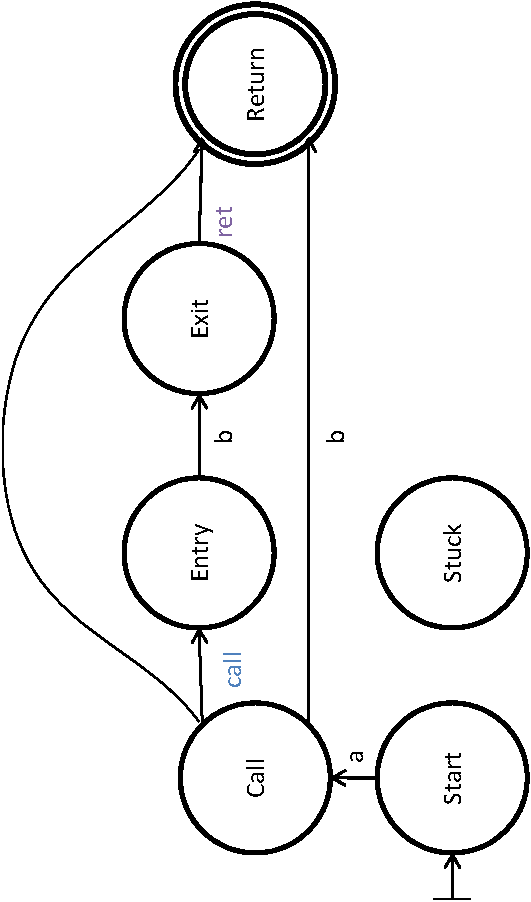
\includegraphics[angle=270,width=10cm]{Figures/Figure13.pdf}
%  \caption{Complex NWA on which to perform Kleene-Star.}
%  \label{Fi:Star3}
%\end{figure}

%\begin{figure}[htbp]
%  \centering
%    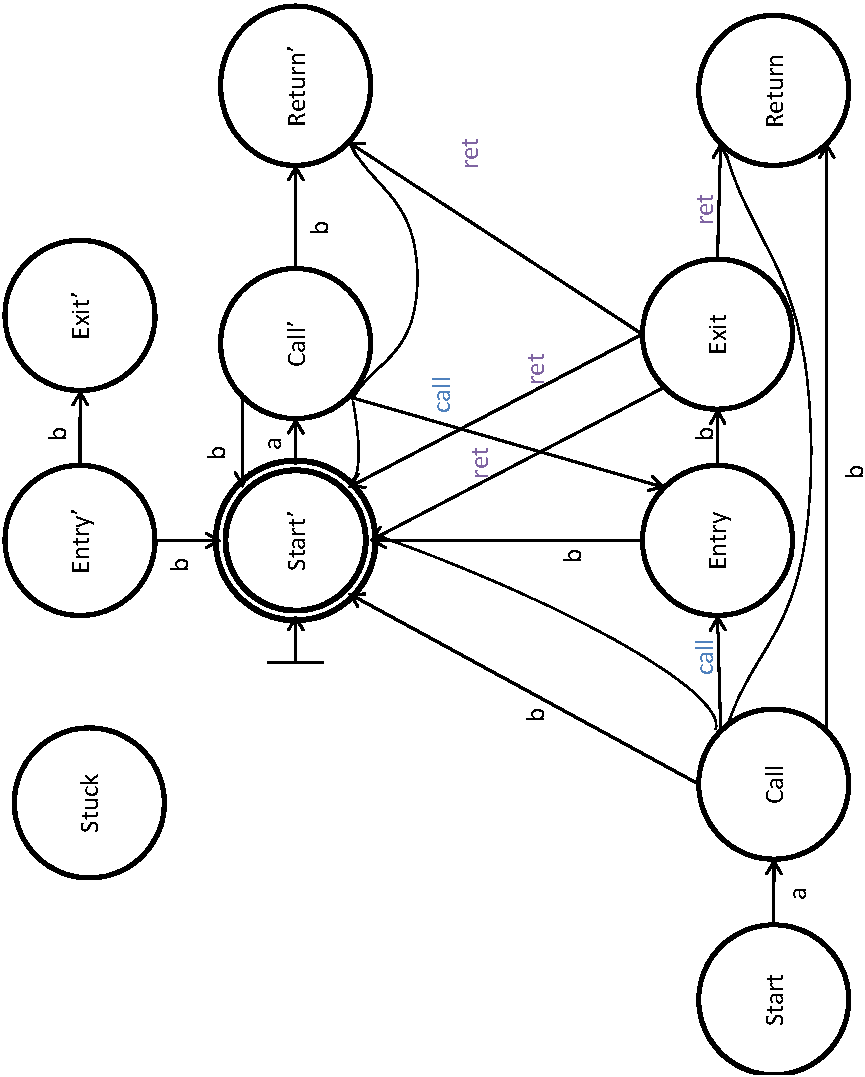
\includegraphics[angle=270,width=12cm]{Figures/Figure14.pdf}
%  \caption{The NWA resulting from performing Kleene-Star on the NWA in Figure \ref{Fi:Star3}.}
%  \label{Fi:Star4}
%\end{figure}

\subsection{Reverse}
\label{Se:Reverse}



If the original NWA is $(Q, \Sigma, Q_0, \delta, Q_f)$, then the result of
reversing that NWA is $(Q, \Sigma, Q_f, \delta_{rev}, Q_0)$ obtained using
the following rules:

\begin{mathpar}
{\inferrule*[left=\textsc{Internal}]
     { (q,\sigma,q') \in \delta_i  }
  { (q',\sigma,q)  \in {\delta_{rev}}_i }
} 
\and
{\inferrule*[left=\textsc{Call}]
       { (q_c,\sigma,q_e) \in \delta_c }
  { (q_e,\sigma,q_c) \in {\delta_{rev}}_c }
}
\and
{\inferrule*[left=\textsc{Return}]
  { (q_x,q_c,\sigma,q_r) \in \delta_r  \\ (q_c,\sigma,q_e) \in  \delta_c }
  { (q_r,q_e,\sigma,q_x) \in {\delta_{rev}}_r }
}
\end{mathpar}


The NWA resulting from performing reverse on the NWA shown in
Figure \ref{Fi:Example1} is shown in Figure \ref{Fi:Reverse1}.
 

Client
information is copied directly from the original NWA using
\texttt{ClientInfo::clone()}.

\subsection{Determinize}
\label{Se:Determinize}

\begin{definition}
An NWA, $(Q,\Sigma,Q_0,\delta,Q_f)$, is \textbf{deterministic} iff 

\begin{enumerate} 

\item $|Q_0| = 1$, 

\item For all $q \in Q$, there is never a choice between reading $\sigma$ and
  following a $\sigma$ transition or following a \wild\ transition:
  \begin{itemize}
    \item if $(q,\wild,q') \in \delta_i$ then $|\{q'|(q,\sigma,q') \in
      \delta_i, {\sigma\neq*}\}| = 0$; \\ otherwise, for all $\sigma \in \Sigma - \{\wild\}$,
      $|\{q'|(q,\sigma,q') \in \delta_i\}| \leq 1$,

    \item if $(q,\wild,q') \in \delta_c$ then $ |\{q'|(q,\sigma,q') \in
      \delta_c, {\sigma\neq*}\}| = 0$;\\
      otherwise, for all $\sigma \in \Sigma - \{\wild\}$,
      $|\{q'|(q,\sigma,q') \in \delta_c\}| \leq 1$, and

    \item for $q' \in Q$, if $(q,q',\wild,q'') \in \delta_r$ then
      $|\{q''|(q,q',\sigma,q'') \in \delta_r, {\sigma\neq*}\}| = 0$; \\
      otherwise, for all
      $\sigma \in \Sigma - \{\wild\}$, $|\{q''|(q,q',\sigma,q'') \in \delta_r\}|
      \leq 1$,
  \end{itemize}
\item And there are no $\epsilon$ transitions:
 \begin{itemize}
   \item for all $(q,\sigma,q') \in \delta_i, \sigma \neq \epsilon$,
   \item for all $(q,\sigma,q') \in \delta_c, \sigma \neq \epsilon$, and
   \item for all $(q,q',\sigma,q'') \in \delta_r, \sigma \neq \epsilon$.
 \end{itemize}
\end{enumerate}
If an NWA is not deterministic, then it is \textbf{non-deterministic}.
\end{definition}

Determinizing an NWA operates like a
generalization of the classical subset construction.  Instead of the states
in the determinized NWA being subsets of states in the original NWA, states of the
determinized NWA are sets of state pairs (i.e., binary relations on states)
\cite{JACM:AM2009}.  To support determinization, the library provides a
typedef of \texttt{std::set$<$pair$<$State, State$>>$} as 
\texttt{NWA::BinaryRelation}. See also \texttt{wali/nwa/RelationOps.hpp}.

We present the algorithm we use for determinization in
\appref{DeterminizeAlgorithm}.

%There is very experimental support for using the BuDDY


The result of determinizing the automaton in \figref{Det1} is shown in
\figref{Det2}.

\begin{figure}[p]
  \centering
    \nwaimage[0.45]{Figures/determinize}
  \caption{Simple nondeterministic NWA.}
  \label{Fi:Det1}
\end{figure}


\begin{figure}[p]
  \centering
    \nwaimage[.75]{Figures/determinize-result}
    \caption{The NWA resulting from determinizing the NWA in Figure
      \ref{Fi:Det1}. As mentioned in the text, states in the determinized NWA
      are relations on the states in the original NWA. The state
      $\varnothing$ has been removed from this diagram.} 
  \label{Fi:Det2}
\end{figure}


Client information is generated through the use of the helper method
\texttt{mergeClientInfo}, but can be altered through the use of the helper
methods \texttt{mergeClientInfoInternal}, \texttt{mergeClientInfoCall}, and
\texttt{mergeClientInfoReturn}, which are invoked by \texttt{determinize} as
transitions of the three kinds involving the associated state are added.  The
default behavior of \texttt{mergeClientInfo} is that the \texttt{ClientInfo}
associated with the resulting state is \texttt{null}.  The default behavior
of \texttt{mergeClientInfoInternal}, \texttt{mergeClientInfoCall}, and
\texttt{mergeClientInfoReturn} is to make no changes to the the
\texttt{ClientInfo}.  These methods can be overridden to specify alternative
behaviors.  As determinization is performed, \texttt{mergeClientInfo} is
called each time a new state is created.  Then, as each transition is added,
\texttt{mergeClientInfoInternal}, \texttt{mergeClientInfoCall}, or
\texttt{mergeClientInfoReturn} is called (depending on the type of transition
being added) to update the \texttt{ClientInfo} associated with the target
state of the transition being added.

The following functions can be overridden in a subclass of \texttt{NWA} to
customize the behavior of determinization:
\begin{functionlist}
  \functionitem[\texttt{void mergeClientInfo(
     \parbox[t]{4in}{
       NWA const \& nondet, BinaryRelation const\& binRel, \\
       St resSt, ref\_ptr<ClientInfo>\& resCI)}}]
  Callback that gets called when a new state \texttt{resSt} (representing the
  binary relation \texttt{binRel}) is added to the determinized automaton.
  Intended to provide a hook for computing the client information that should
  be associated with the new state; the client information should be set in
  the output parameter \texttt{resCI} (i.e. \texttt{setClientInfo} should not
  be called directly). \texttt{nondet} is the NWA being determinized.

  \functionitem[\texttt{void mergeClientInfoInternal(
     \parbox[t]{4in}{
       NWA const \& nondet,\\
       BinaryRelation const\& binRelSource,\\
       BinaryRelation const\& binRelTarget,\\
       Key sourceSt, Key resSym, Key resSt,\\
       ref\_ptr<ClientInfo>\& resCI )}}]
  \functionitem[\texttt{void mergeClientInfoCall(
     \parbox[t]{4in}{
       NWA const \& nondet,\\
       BinaryRelation const\& binRelCall,\\
       BinaryRelation const\& binRelEntry,\\
       Key callSt, Key resSym, Key resSt,\\
       ref\_ptr<ClientInfo>\& resCI )}}] \nopagebreak
  \functionitem[\texttt{void mergeClientInfoReturn(
     \parbox[t]{4in}{
       NWA const \& nondet,\\
       BinaryRelation const\& binRelExit,\\
       BinaryRelation const\& binRelCall,\\
       BinaryRelation const\& binRelReturn,\\
       Key exitSt, Key callSt, Key resSym,\\
       Key resSt, ref\_ptr<ClientInfo>\& resCI )}}]
    Callback that gets called when a new transition is added to the given
    automaton. The endpoints and their associated binary relations are
    given.
    Alters the client information associated with \texttt{resSt} given
    information about the transition being added to the determinized
    automaton.
 \end{functionlist}

%Consider the slightly more complex determinization of the NWA shown in Figure \ref{Fi:Det3}.  The resulting NWA is shown in Figure \ref{Fi:Det4}.

%\begin{figure}[htbp]
%  \centering
%    \includegraphics[angle=270,width=12cm]{Figures/Figure18.pdf}
%  \caption{Complex nondeterministic NWA.}
%  \label{Fi:Det3}
%\end{figure}

%\begin{figure}[htbp]
%  \centering
%    \includegraphics[angle=270,width=12cm]{Figures/Figure19.pdf}
%  \caption{The NWA resulting from determinizing the NWA in Figure \ref{Fi:Det3}.}
%  \label{Fi:Det4}
%\end{figure}

\subsection{Complement}
\label{Se:Complement}

Complementing an NWA is performed by determinizing the automaton then
complementing the set of final states. In our implementation, an extra flag
to \texttt{complement} controls whether the determinization step is
performed, so it can be bypassed if you have \textsl{a priori} knowledge that
the input NWA must already be deterministic. The result of
complementing of the NWA shown in Figure \ref{Fi:Det1} is
shown in Figure \ref{Fi:Comp1}.

Client information is copied directly
from the determinization of the original NWA using \texttt{ClientInfo::clone()}.

\begin{figure}[h]
  \centering
    \nwaimage[1]{Figures/complement-of-determinize}
  \caption{The complement of the NWA in Figure \ref{Fi:Det1} (the
    determinization of which is shown in Figure \ref{Fi:Det2}).  We omit
    transitions to the state $\{\}$; any action which does not appear in that
    diagram goes to that state.
  }
  \label{Fi:Comp1}
\end{figure}



